\documentclass[12pt, a4paper]{article}
\setlength{\parindent}{0pt}
\usepackage[utf8]{inputenc}
\usepackage[spanish]{babel}
\usepackage{hyperref}
\usepackage{graphicx}
\usepackage{wrapfig}
\usepackage{caption}
\usepackage{subcaption}
\usepackage{multirow} 
\usepackage{ amssymb }
\usepackage{amsmath}

\begin{document} 
\title{Trabajo Práctico 4\\ Machine Learning} 
\author{Bianchi, Gabina Luz} 
\maketitle

\section*{Ejercico A}
En este ejercicio se pide implementar el clasificador \textit{k} vecinos más cercanos. El código correspondiente se encuentra en el archivo \textit{ejercicioA.c}.

\section*{Ejercicio B}
 
En este ejercicio se pide resolver el problema de las espirales anidadas con el clasificador de primer vecino. En la Figura 1 se grafica la predicción en los 2000 puntos de test. El error porcentual en dicho conjunto se encuentra entre el 5\% y el 6\%. Es esperable que clasifique correctamente ya que los puntos en general están pegados o más cercanos a puntos de su misma clase, a excepción de aquellos que se encuentran en el límite de las espirales. Posiblemente, únicamente en ellos esté fallando.\\
En la Figura 2 se presenta una tabla con los resultados para redes neuronales, en función de la cantidad de neuronas utilizadas en la capa intermedia. Allí se puede observar que el resultado para primer vecino es comparable con el mejor que se logró con redes. \\
Si bien el problema de las espirales anidadas no es simple en general (por ejemplo, para las redes neuronales), es la clase de problemas que el clasificador del primer vecino puede afrontar. Las clases tienen formas complejas, pero continuas, y no hay ruido. Por lo tanto, mirar el primer vecino para decidir es suficiente, y de hecho, si se tiene en cuenta una mayor cantidad de puntos cercanos, la predicción no es capaz de mantener la complejidad de las figuras.
 
 \begin{figure}
    \centering
	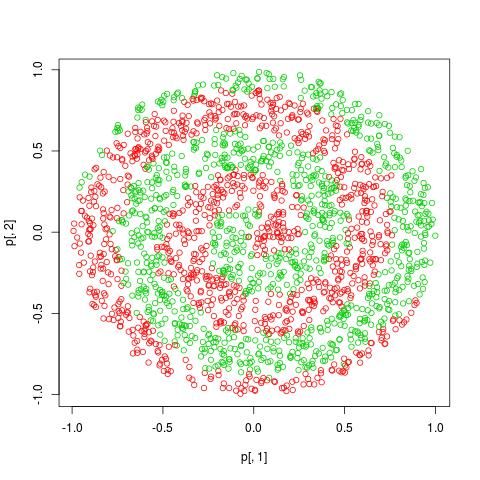
\includegraphics[scale=0.4]{espirales12}
	\caption{Predicción para espirales anidadas utilizando el clasificador de primer vecino.}
\end{figure}

 \begin{figure}
    \centering
	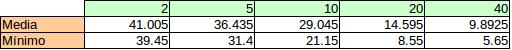
\includegraphics[scale=1]{tablaB}
	\caption{Error porcentual para espirales anidadas con redes neuronales, variando el número de neuronas en la capa intermdia.}
\end{figure}


\section*{Ejercicio C}

En este ejercicio se pide resolver el problema de las gaussianas diagonales y paralelas, variando las dimensiones, con el clasificador \textit{k} primeros vecinos. Para elegir la cantidad de vecinos óptima, se hizo un barrido con 1, 2,	5,	10, 15, 30, 50, 80, 90, 100 y 150 vecinos, y se eligió en función del error en el conjunto de validación. Los menores errores en validación se encuentran al considerar entre los 50 y los 100 vecinos más cercanos, dependiendo de la cantidad de dimensiones. En la Figura 3 se presentan los errores porcentuales en test para el problema de dimensionalidad con todos los clasificadores vistos hasta ahora, el clasificador de primer vecino, y el de 80 vecinos, el cual fue considerado en general el óptimo. Allí se puede apreciar, por un lado, que los problemas diagonal y paralelo no presentan grandes diferencias, lo cual parece razonable para este caso. Por el otro, que el clasificador de primer vecino no logra buenos resultados, y que éstos empeoran considerablemente con el aumento de las dimensiones. Por el contrario, el clasificador de 80 primeros vecinos logra muy buenos resultados, únicamente siendo superado por el clasificador Naive Bayes, y parece ser resistente al aumento de dimensiones.

 \begin{figure}
    \centering
	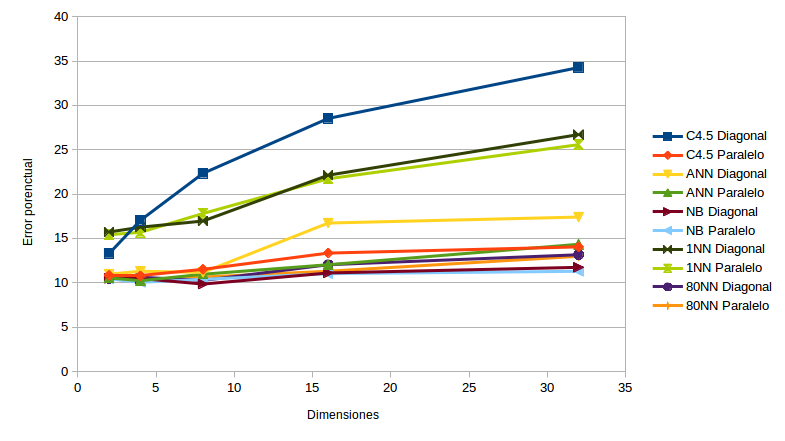
\includegraphics[scale=0.8]{ejercicioc}
	\caption{Error porcentual en función de las dimensiones para las gaussians paralelas y diagonales, utilizando distintos clasificadores.}
\end{figure}

En la Figura 4 se presentan las predicciones para 2 dimensiones de las gaussianas diagonales, utilizando 1 vecino y 80. Allí se puede explicar por qué el clasificador del primer vecino no es bueno para este caso. Hay sectores en los cuales las clases están muy mezcladas, y considerar únicamente el primer vecino conlleva muchas veces a una clasificación incorrecta. Como se vio en el ejercicio anterior, el clasificador de primer vecino tiene tendencia a encontrar clases complejas, mientras que un clasificador que considera más puntos cercanos, tiende a encontrar figuras más generales, ya que mira la tendencia a su alrededor y no un punto en particular, lo cual lo hace más resistente al ruido. Por lo tanto, para un caso como el de las gaussianas paralelas y diagonales, es más apropiado un clasificador que considere un número mayor de vecinos.

\begin{figure}
    \centering

    \begin{subfigure}[b]{0.45\textwidth}
        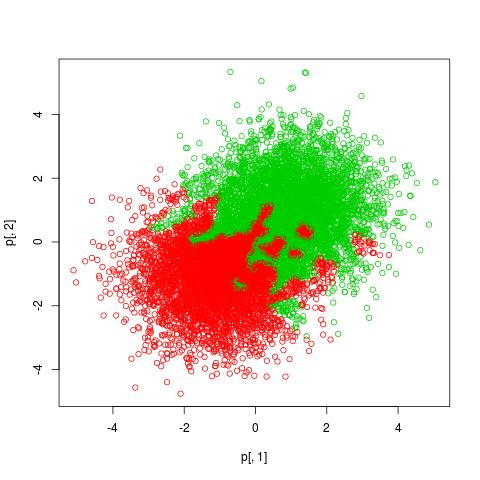
\includegraphics[width=\textwidth]{pred1vecino}
        \caption{Utilizando 1 vecino}
        %\label{fig:tiger}
    \end{subfigure}
      ~ %add desired spacing between images, e. g. ~, \quad, \qquad, \hfill etc. 
      %(or a blank line to force the subfigure onto a new line)
    \begin{subfigure}[b]{0.45\textwidth}
        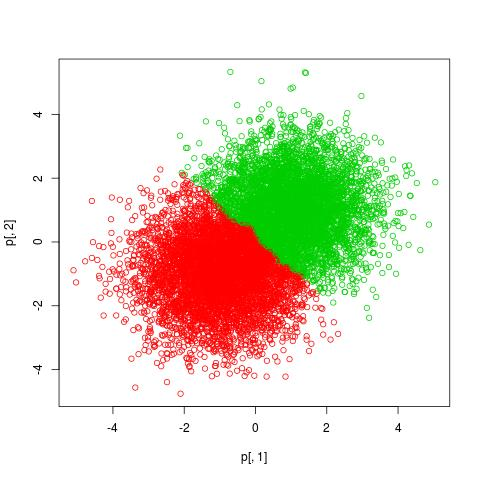
\includegraphics[width=\textwidth]{pred80vecino}
        \caption{Utilizando 80 vecinos}
        %\label{fig:gull}
    \end{subfigure}
    \caption{Predcciones para gaussianas diagonales de 2 dimensiones, variando la cantidad de vecinos más cercanos utilizados.}
\end{figure}


\section*{Ejercicio D}
En este ejercicio se pide implementar una modificación al algoritmo de \textit{k} vecinos más cercanos. En lugar de utlizar una cantidad fija de puntos, se fija una distancia \textit{d} y se miran todos los vecinos que se encuentran a una distancia menor que ella. El código correspondiente se encuentra en el archivo \textit{ejercicioD.c}.

\bigskip

Al aplicar este clasificador al problema de la dimensionalidad, ocurre que para una distancia fija \textit{d} la cantidad de puntos que se tienen en cuenta no es la misma, según la dimensión y según la desviación estándar de las gaussianas. En particular, en el caso de las gaussianas diagonales, la desviación estándar depende de la cantidad de dimensiones. Por lo tanto, para las gaussianas diagonales de 32 variables, se necesita una distancia mucho mayor para mirar una cantidad de vecinos alta, que para los otros casos. En la Figura 5 se presenta la gráfica con los resultados de error porcentual. Se puede observar que la clasificación utilizando distancia 3, comienza siendo buena, pero al aumentar las dimensiones, se empareja con 1NN. A su vez, si se fija la distancia en 30, únicamente se obtiene un buen resultado para la gaussiana diagonal de 32 dimensiones.\\
Por lo tanto, se puede conluír que es preferible fijar la cantidad de vecinos a tener en cuenta, que la distancia máxima. 

 \begin{figure}
    \centering
	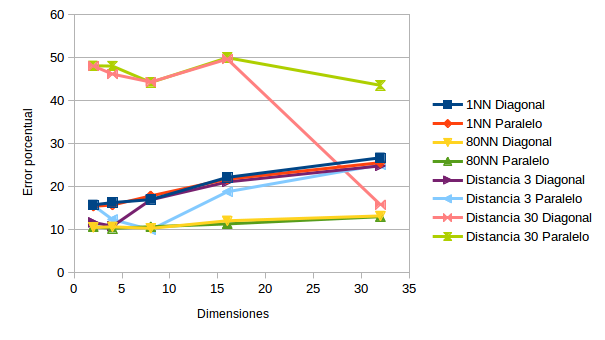
\includegraphics[scale=0.8]{ejerciciod}
	\caption{Error porcentual en función de las dimensiones para las gaussians paralelas y diagonales, utilizando distintos clasificadores.}
\end{figure}

\section*{Ejercicio E}

En este ejercicio se pide pensar sobre el sobreajuste en \textit{k} vecinos más cercanos. El análisis se limitó únicamente a dos dimensiones y dos clases. Cuando se aplicó el algoritmo del primer vecino a las gaussianas, se presentaba un claro ejemplo de sobreajuste, ya que el error en entrenamiento siempre daba 0\%. Esto es debido a que, para cada punto de entrenamiento, siempre existe un punto de entrenamiento a distancia cero (él mismo), que lo clasifica bien. Ahora se pide analizar si puede haber sobreajuste, cuando el mismo punto que se está ajustando, no es tenido en cuenta. \\
Según lo analizado en los ejercicios anteriores, se puede concluír que el clasificador del primer vecino es fácilmente influenciable. Por lo tanto, es esperable que el sobreajuste se dé por usar pocos vecinos, generando clases complejas, cuando en realidad éstas son simples. \\
Considerando entonces que el clasificador de primer vecino es un gran consumidor de ruido, la primera idea que surge para producir sobreajuste, es darle un conjunto de datos de entrenamiento que posea ruido. Sin embargo, si el ruido consta de puntos aislados mal clasificados, el error en entrenamiento también es alto (porque clasifica mal el ruido). Por lo tanto necesitamos un ruido particular en el cual haya varias regiones de puntos cercanos mal clasificados. \\
Para el ejemplo se optó por un conjunto de datos con clases muy simples, y un conjunto de entrenamiento que confunda. Ambos se grafican en la Figura 6. Entonces, la idea es que al utilizar pocos vecinos para clasificar, el error en entrenamiento sea bajo y el de test alto, porque se capta muy bien el ruido. Al aumentar la cantidad de puntos cercanos que se tienen en cuenta, el algoritmo logra que los puntos mal clasificados del entrenamiento, no le influyan en su decisión. De esta manera, el error en entrenamiento y en test se invierten.\\
En la Figura 7 se grafican las predicciones según la cantidad de vecinos utilizadas, y en la Figura 8, los errores porcentuales en test y entrenamiento.
\begin{figure}
    \centering

    \begin{subfigure}[b]{0.45\textwidth}
        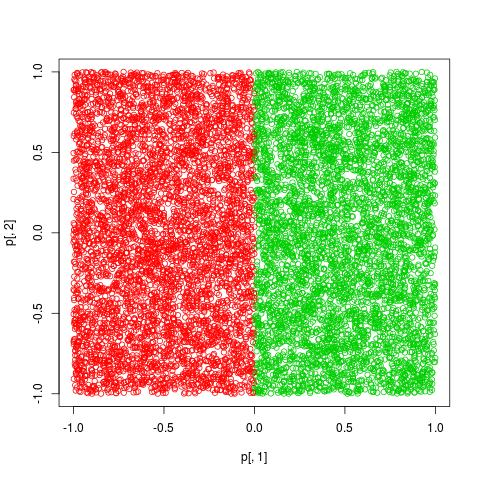
\includegraphics[width=\textwidth]{testE}
        \caption{Conjunto de test con 10000 puntos}
        %\label{fig:tiger}
    \end{subfigure}
      ~ %add desired spacing between images, e. g. ~, \quad, \qquad, \hfill etc. 
      %(or a blank line to force the subfigure onto a new line)
    \begin{subfigure}[b]{0.45\textwidth}
        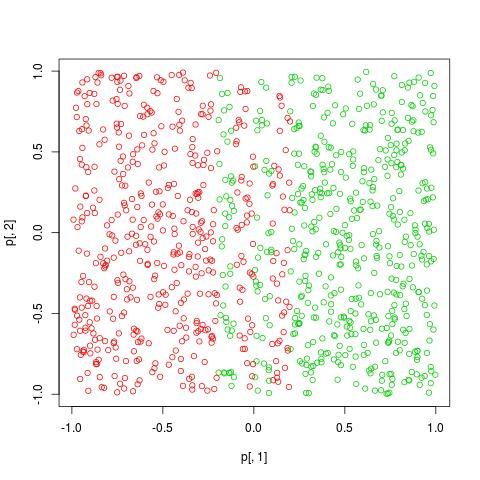
\includegraphics[width=\textwidth]{datosE}
        \caption{Conjunto de entrenamiento con 1000 puntos}
        %\label{fig:gull}
    \end{subfigure}
    \caption{Puntos utilizados para generar sobreajuste.}
\end{figure}

\bigskip

\begin{figure}
    \centering

    \begin{subfigure}[b]{0.45\textwidth}
        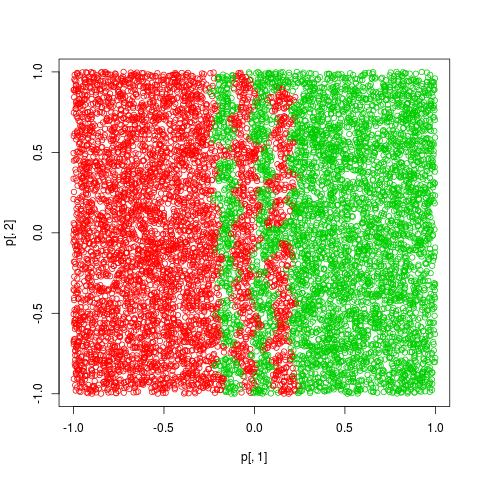
\includegraphics[width=\textwidth]{predE1}
        \caption{Utilizando 1 vecino}
        %\label{fig:tiger}
    \end{subfigure}
    \begin{subfigure}[b]{0.45\textwidth}
        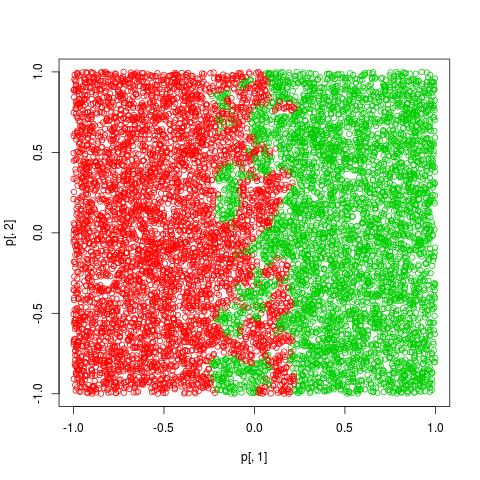
\includegraphics[width=\textwidth]{predE10}
        \caption{Utilizando 10 vecinos}
        %\label{fig:tiger}
    \end{subfigure}
      ~ %add desired spacing between images, e. g. ~, \quad, \qquad, \hfill etc. 
      %(or a blank line to force the subfigure onto a new line)
    \begin{subfigure}[b]{0.45\textwidth}
        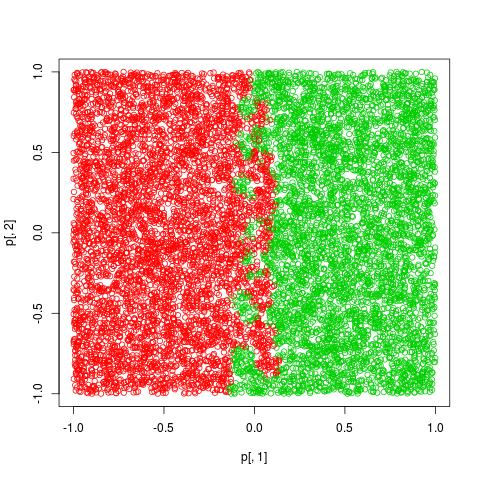
\includegraphics[width=\textwidth]{predE30}
        \caption{Utilizando 30 vecinos}
        %\label{fig:gull}
    \end{subfigure}
    \begin{subfigure}[b]{0.45\textwidth}
        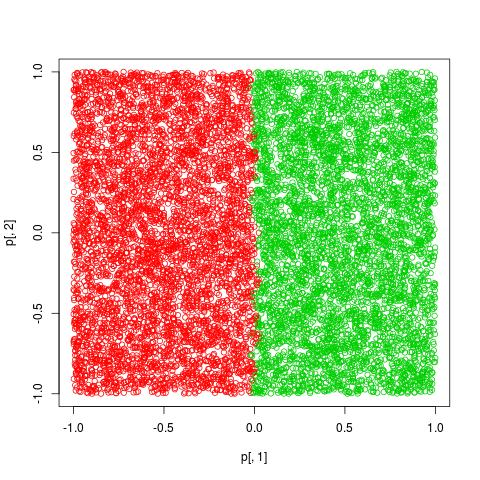
\includegraphics[width=\textwidth]{predE60}
        \caption{Utilizando 60 vecinos}
        %\label{fig:tiger}
    \end{subfigure}        
    \caption{Predicciones para el conjunto de test según la cantidad de vecinos utilizados}
\end{figure}

 \begin{figure}
    \centering
	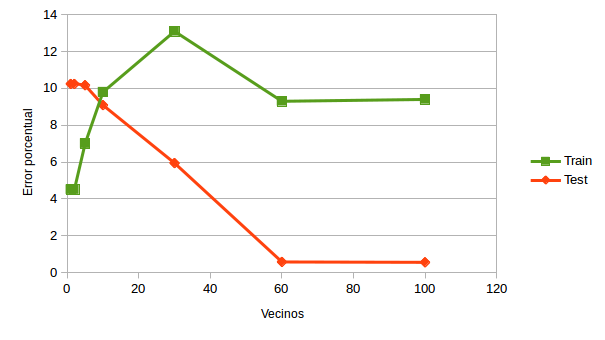
\includegraphics[scale=0.8]{ejercicioe}
	\caption{Error porcentual en entrenamiento y test según la cantidad de vecinos utilizados.}
\end{figure}

\bigskip


\end{document}